\documentclass[twocolumn,13pt]{article}
\usepackage{graphicx}
\usepackage[utf8]{inputenc}
\usepackage{hyperref}



\begin{document}
\title{\textbf{printing sum of two numbers on LCD}}

\author{kanekal kousar}
\date{\today}
\maketitle

 \section{Abstract}-Through this manual, we learn how to display sum of two numbers on LCD


\section{components}


\begin{tabular}{ |p{3cm}|p{1.5cm}|p{1.5cm}| }
 \hline
 \setlength{\tabcolsep}{3pt}
components & values & quantity \\
\hline
 Resistor  & 220ohm    &1\\
 Arduino &   UNO & 1\\
 LCD &16x2 & 1\\
 bread board  &-& 1\\
 jump wires&  - & 20\\
 \hline
\end{tabular}
\begin{center}
    TABLE I
\end{center}
 

\section*{step 1}
-Connect the 5V pin of the Arduino to an extreme pin of the Breadboard
Let this pin be V cc .
\section*{step 2}
-Connect the GND pin of the Arduino to the opposite extreme pin of the Breadboard.
\section*{step 3}
-plug the LCD in fig.7 to breadboard
\section*{step 4}
-Connect the 220Ohm resistance from Vcc to pin 15 (Led+) of the LCD.
\section*{step 5}
-Connect the arduino to the computer so that it is powered.

\begin{center}
    TABLE II :Arduino to LCD connections
\end{center}
 \begin{tabular}{ |p{1.5cm}|p{1.5cm}|p{1.5cm}|p{1.5cm}| }
 \hline
 \setlength{\tabcolsep}{3pt}
Arduino pins & LCD pins & LCD pin label & LCD pin Description\\
\hline
 GND & 1& GND & \\
 \hline
 5V & 2 & Vcc &\\
 \hline
 GND & 3 & Vee & Contrast\\
 \hline
 D6 & 4 & RS & Register Select\\
 \hline
 GND & 5 & R/W & read/write\\
 \hline
 D7 & 6 & EN &Enable\\
 \hline
 D2 & 11 & DB4 & Serial connection\\
 \hline
 D3 & 12 & DB5 & Serial connection\\
 \hline
 D4 & 13 & DB6 & Serial connection\\
 \hline
 D5 & 14 & DB7 & Serial connection\\
 \hline
 5V & 15 & LED+ & Backlight\\
 \hline
 GND & 16 & LED- & Backlight\\
 \hline
\end{tabular}



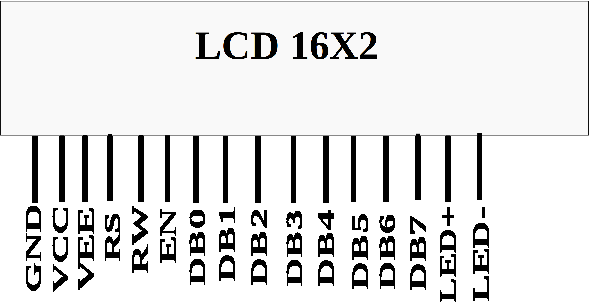
\includegraphics[scale=0.3]{../assembly_assignment/figs/lcd.png} 




\section*{step 6}
-make the Arduino to LCD pin connections as show in  table II
\section*{step 7}
-Open the Arduino IDE and type the following code.
\framebox{
\url{https://github.com/kkousar/KOUSAR_FWC/blob/main/assembly_assignment/lcd_code/lcd_code.asm}}
\bibliographystyle{ieeetr}
\section*{Result}
-on LCD display you will get the sum of numbers 



\end{document}


